\documentclass{article}
\usepackage{graphicx} % Required for inserting images
\usepackage{fancyhdr} % Required for header and footer configuration
\usepackage[a4paper, margin=2.5cm, left=1.5cm, right=1.5cm, bottom=4cm]{geometry} % Required for setting page margins
\usepackage[T1]{fontenc}
\usepackage[default,oldstyle,scale=1]{opensans} % Utilizzo del font Open Sans
\usepackage{lipsum} 
\usepackage{makeidx}
\usepackage{booktabs}
\usepackage{tabularray}
\usepackage[colorlinks=true, linkcolor=black, urlcolor=blue, citecolor=blue]{hyperref}
\usepackage{tabularx}
\usepackage{makecell}

% Configure header and footer for the first page
\fancypagestyle{firstpage}{
    \fancyhf{} % Clear header and footer
    \renewcommand{\headrulewidth}{0pt} % Remove header rule line
    \lhead{} % Header on the left
    \chead{} % Header in the center
    \rhead{} % Header on the right
    \lfoot{} % Footer on the left
    \cfoot{\vspace{5pt}\\\hrulefill\\\vspace{10pt}\textbf{BeeLive}\\Gruppo 21} % Footer in the center
    \rfoot{\vspace{32.5pt}\\\thepage} % Footer on the right
}

% Configure header and footer for non-plain pages (second page onwards)
\fancypagestyle{nonplain}{
    \fancyhf{} % Clear header and footer
    \lhead{} % Header on the left
    \chead{} % Header in the center
    \rhead{
\includegraphics[width=2cm]{Images/BeeLive-Logo.png}\\\vspace{2pt}} % Header on the right
    \lfoot{} % Footer on the left
    \cfoot{\vspace{5pt}\\\hrulefill\\\vspace{10pt}\textbf{BeeLive}\\Gruppo 21} % Footer in the center
    \rfoot{\vspace{32.5pt}\\\thepage} % Footer on the right
}

% Adjust vertical space between header and text
\setlength{\headsep}{65pt} 
% Adjust vertical space between text and footer
\setlength{\footskip}{0pt} 

\title{
\includegraphics[width=0.75\textwidth]{Images/BeeLive-Logo.png}\\\vspace{100pt}
\LARGE{\textbf{BeeLive\\Deliverable 1}}}
\author{Gruppo 21:\\
Cipriani Pietro, 226959\\
Orlando Dennis, 227688\\
Ziviani Elia, 228172}
\date{28 Marzo 2024}

\makeindex % Indica che vogliamo creare un indice

\begin{document}

\maketitle
\thispagestyle{firstpage} % Apply firstpage style to the first page
\clearpage

\pagestyle{nonplain} % Apply non-plain style to subsequent pages

\renewcommand{\contentsname}{Indice}
\tableofcontents

\clearpage
\section{Descrizione dell'applicativo}
\index{Descrizione dell'applicativo} % Aggiunge una voce all'indice
La Municipalità di Trento ha richiesto la valutazione dei problemi cittadini e la proposta di soluzioni attraverso lo sviluppo di un'applicazione web ad-hoc.

Dopo un processo di ideazione, è emerso che a Trento risulta spesso difficile reperire informazioni riguardanti gli eventi che influenzano la viabilità stradale. Le informazioni disponibili sono principalmente testuali e richiedono un impegno attivo da parte dei cittadini per essere trovate, poiché attualmente manca un sistema di notifica automatica per tali modifiche.

Di conseguenza, l'idea concepita prevede lo sviluppo di un sistema informativo che consenta ai cittadini di accedere rapidamente ed intuitivamente a tutte le variazioni della viabilità, senza la necessità di una ricerca attiva.\\

Il nucleo concettuale si basa sulla rappresentazione grafica delle zone coinvolte nelle modifiche della viabilità, per facilitare la comprensione delle informazioni.\\
È inoltre previsto un sistema di notifiche push per informare i cittadini in tempo reale sugli eventi che coinvolgono l'intera città o solo le zone da loro selezionate.\\

Saranno sviluppati due ambienti distinti: Uno riservato all'amministrazione e uno accessibile ai cittadini.\\
Il primo ambiente consentirà all'amministrazione di inserire e modificare le informazioni sulle variazioni della viabilità attraverso un'interfaccia grafica intuitiva e compatibile con gli standard per la visualizzazione dei dati su mappa.\\
Il secondo sarà un'applicazione mobile installabile sui dispositivi dei cittadini, che consentirà loro di visualizzare graficamente le zone interessate dai cambiamenti, selezionare le aree di loro interesse e ricevere notifiche push in tempo reale.

Ogni variazione inserita nel sistema dall'amministrazione sarà caratterizzata dalla zona interessata, visualizzabile sulla mappa, da una descrizione che ne spiega la natura e da una stima della durata della variazione, tutte informazioni che i cittadini potranno visualizzare tramite l'applicazione mobile dal loro dispositivo.
\clearpage

\clearpage

\section{Obiettivi}
\index{Obiettivi} % Aggiunge una voce all'indice

Archiviazione eventi\\


\clearpage

\section{Attori di sistema e Mind map}
\index{Attori di sistema e Mind map} % Aggiunge una voce all'indice

\subsection{Attori di sistema Interni}
\index{Attori di sistema Interni}

\subsubsection{Utente anonimo}\label{Attori_UtenteAnonimo}
\index{Utente anonimo} % Aggiunge una voce all'indice
Si tratta del cittadino che utilizza l'applicativo. Ha accesso a tutte le funzionalità ma non è disponibile la sincronizzazione tra più dispositivi.

\subsubsection{Utente autenticato}
\index{Utente autenticato} % Aggiunge una voce all'indice
L'utente autenticato eredita tutte le caratteristiche dall'utente anonimo (\ref{Attori_UtenteAnonimo}), integrando però la sincronizzazione tra i dispositivi su cui l'utente esegue l'accesso.

\subsubsection{Dipendente autorizzato del Comune di Trento}\label{Attori_DipendenteAutorizzato}
\index{Dipendente del Comune di Trento} % Aggiunge una voce all'indice
Il dipendente autorizzato del Comune di Trento è colui che ha il compito di gestire gli eventi che influenzano la viabilità cittadina.

\subsubsection{Enti delegati}
\index{Enti delegati} % Aggiunge una voce all'indice
Gli enti delegati ereditano le caratteristiche dall'entità "Dipendente autorizzato del Comune di Trento" (\ref{Attori_DipendenteAutorizzato}), essendo però esterno alla gestione comunale del territorio.

\subsubsection{Amministratore di sistema}
\index{Amministratore di sistema} % Aggiunge una voce all'indice
L'entità che si occupa della gestione del sistema, con la possibilità di modificare le policies di access control e definire le aree di competenza delle entità di gestione.

\subsection{Attori di sistema Esterni}
\index{Attori di sistema Esterni}

\subsubsection{Enti delegati}
\index{Enti delegati} % Aggiunge una voce all'indice

\subsection{Componenti di sistema Interni}
\index{Componenti di sistema Interni}
\subsubsection{Applicativo mobile}
\index{Applicativo mobile}

\subsubsection{Applicativo desktop}
\index{Applicativo desktop}

\subsubsection{Web server}
\index{Web server}

Separato in due parti\\
Ogniuna con utenti autenticati

\subsubsection{Database}
\index{Database}

\subsection{Componenti di sistema Esterni}
\index{Componenti di sistema Esterni}

\subsubsection{Server di autenticazione}
\index{Server di autenticazione}

\subsubsection{Server provider}
\index{Server provider}

\clearpage

\subsection{Mind map}
\index{Mind map}

\begin{figure}[htbp]
    \label{fig:Mind_map}
    \centering
    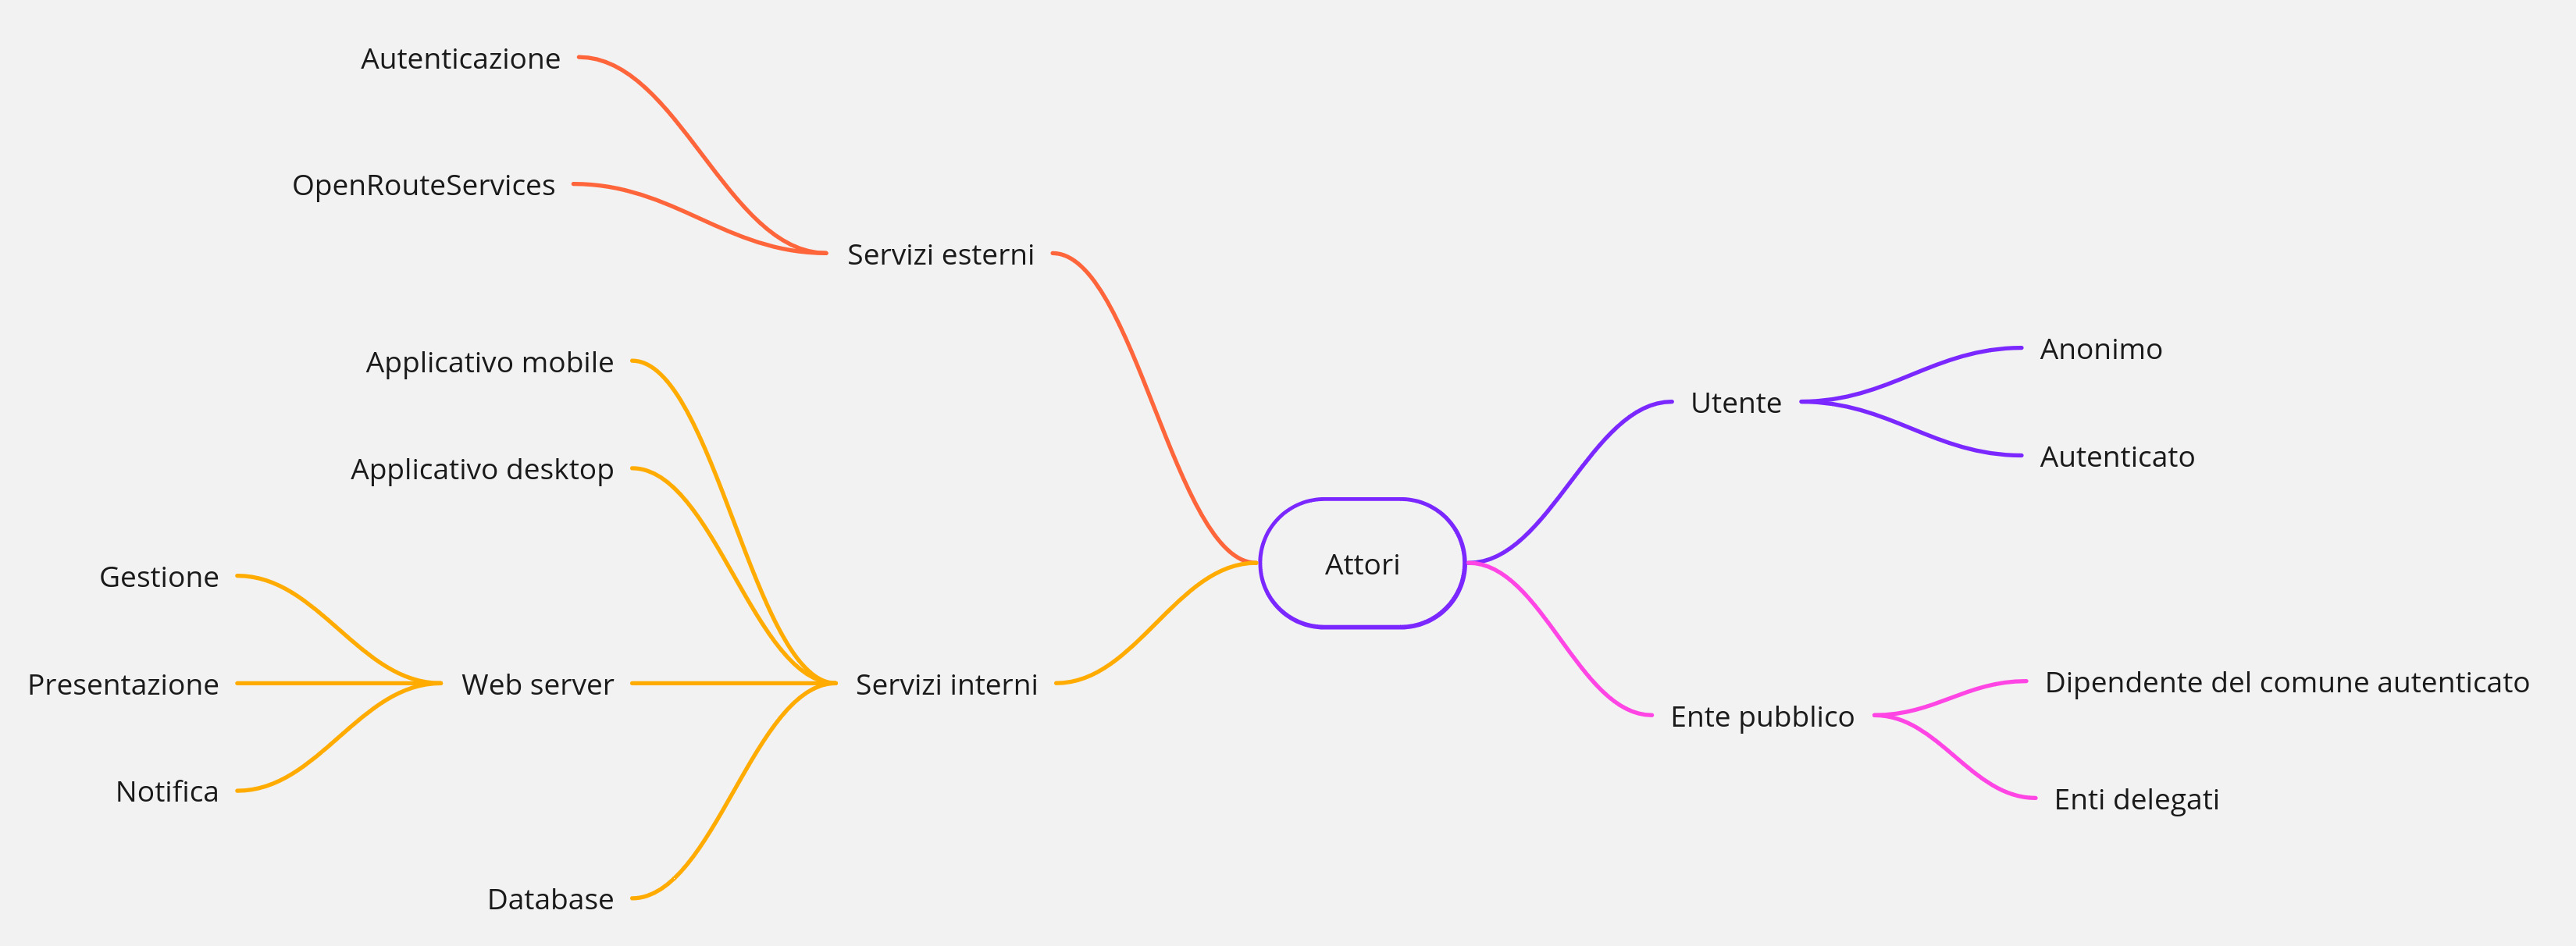
\includegraphics[width=1\textwidth]{Images/BeeLive-MindMap.jpg}
    \caption{Mind map degli attori che interagiscono con il sistema}
\end{figure}

Tramite la mind map è possibile avere una rappresentazione chiara degli attori che interagistocno con il sistema.\\
\clearpage

\section{Prototipo del sistema}
\index{Prototipo del sistema} % Aggiunge una voce all'indice

\subsection{Mockup applicazione mobile}
\index{Mockup applicazione mobile} % Aggiunge una voce all'indice\usepackage{makecell}

\subsubsection{Schermata principale}
\index{Schermata principale} % Aggiunge una voce all'indice
\begin{figure}[htbp]
    \label{fig:Schermata_principale_mobile}
    \centering
    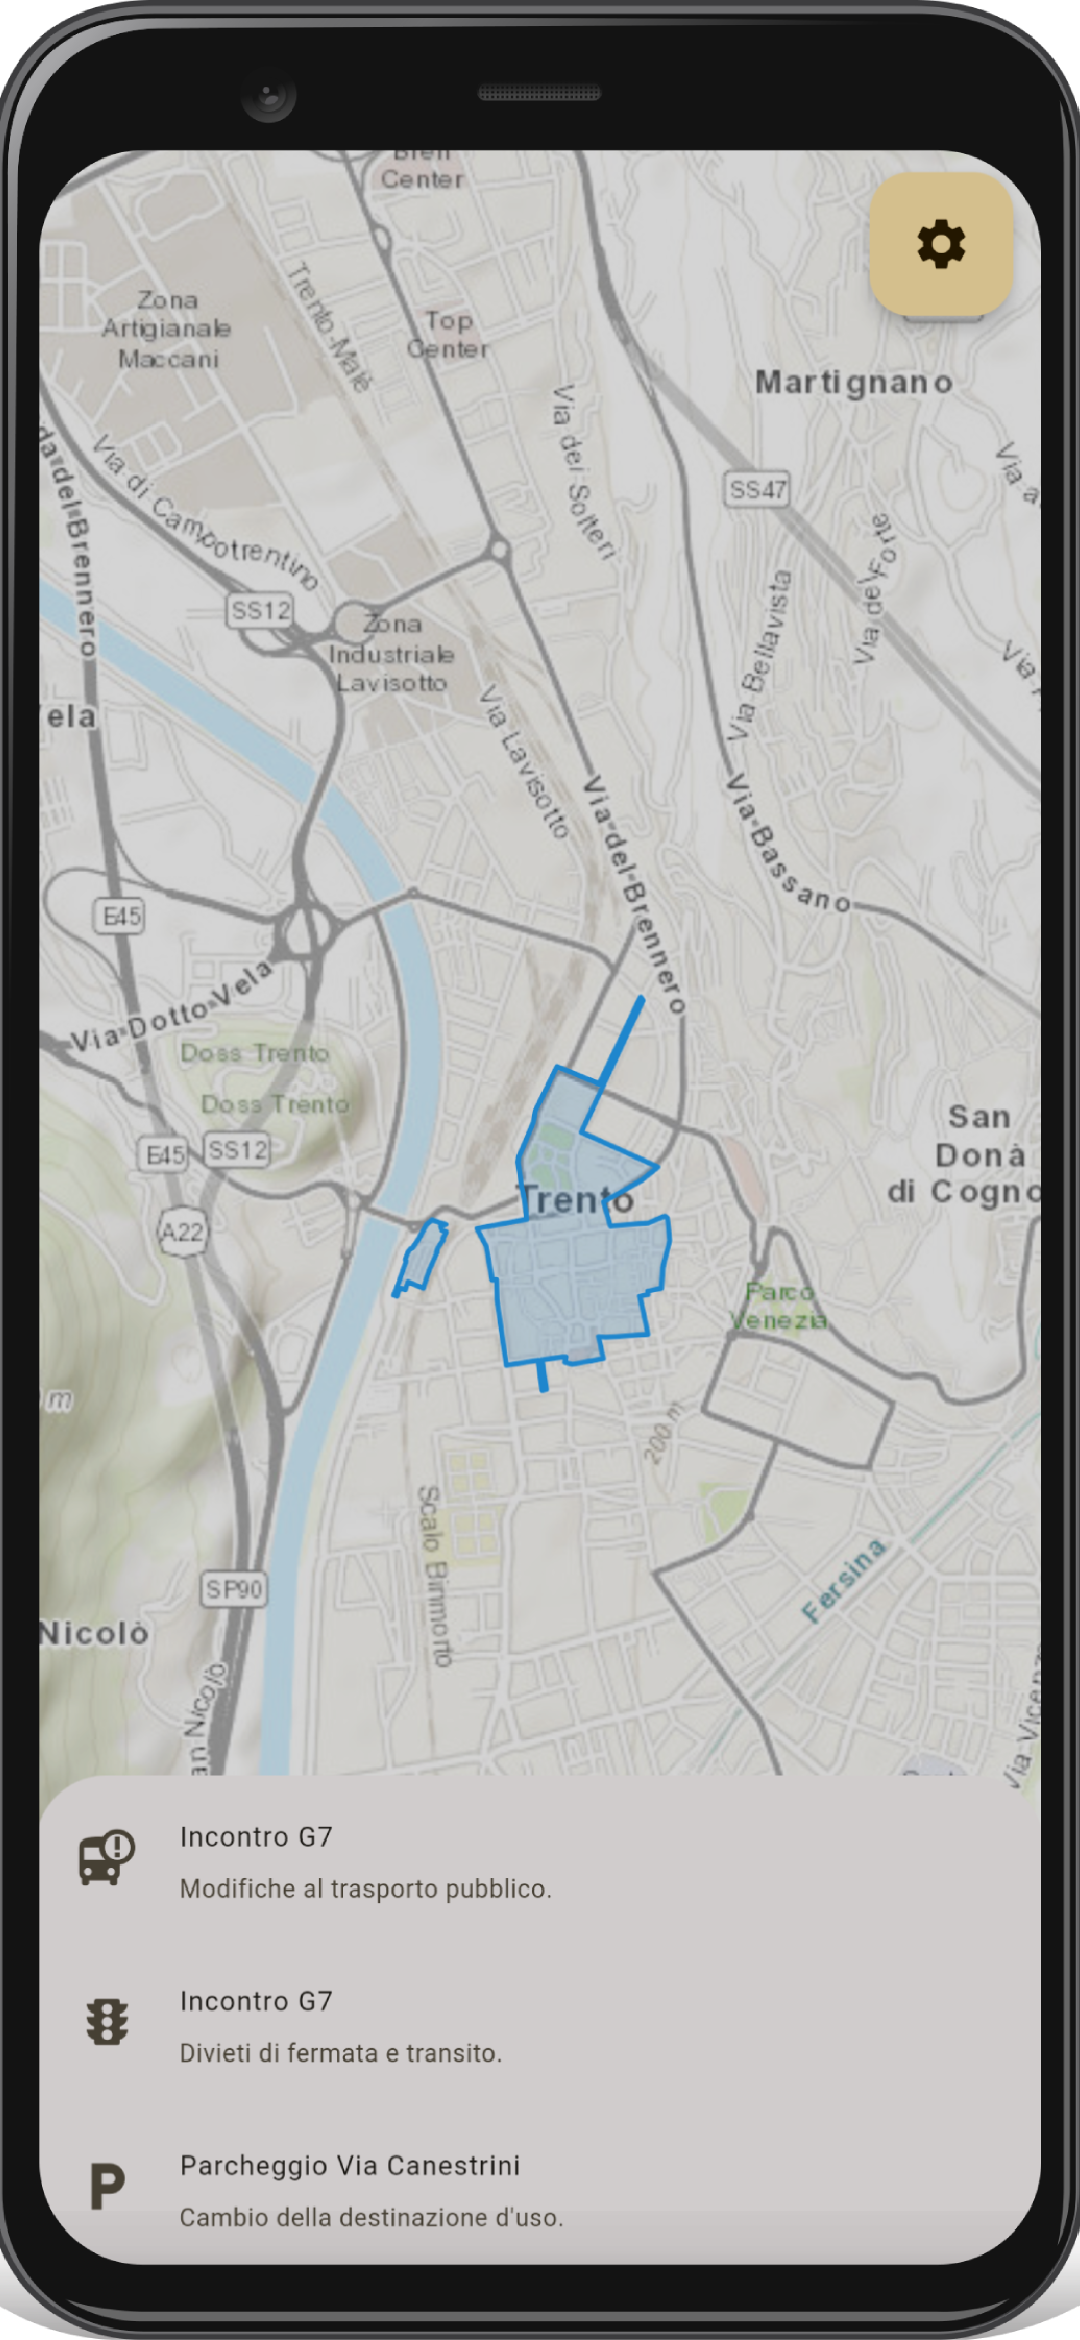
\includegraphics[width=0.25\textwidth]{Images/Mockup1 - Mobile.png}
    \caption{Mockup schermata principale dell'applicazione mobile}
\end{figure}

È rappresentata la schermata principale dell'applicazione mobile che il cittadino installerà sul proprio smartphone.\\
La schermata principale mostra una mappa della città di Trento con le zone interessate dalle variazioni della viabilità.\\
La lista sottostante la mappa riporta tutte le variazioni presenti nel sistema che si trovano nel periodo di visualizzazione, con la possibilità di selezionare una variazione per visualizzarne i dettagli.\\
\clearpage

\subsubsection{Dettagli variazione selezionata}
\index{Dettagli variazione selezionata} % Aggiunge una voce all'indice
\begin{figure}[htbp]
    \label{fig:Dettaglio_evento}
    \centering
    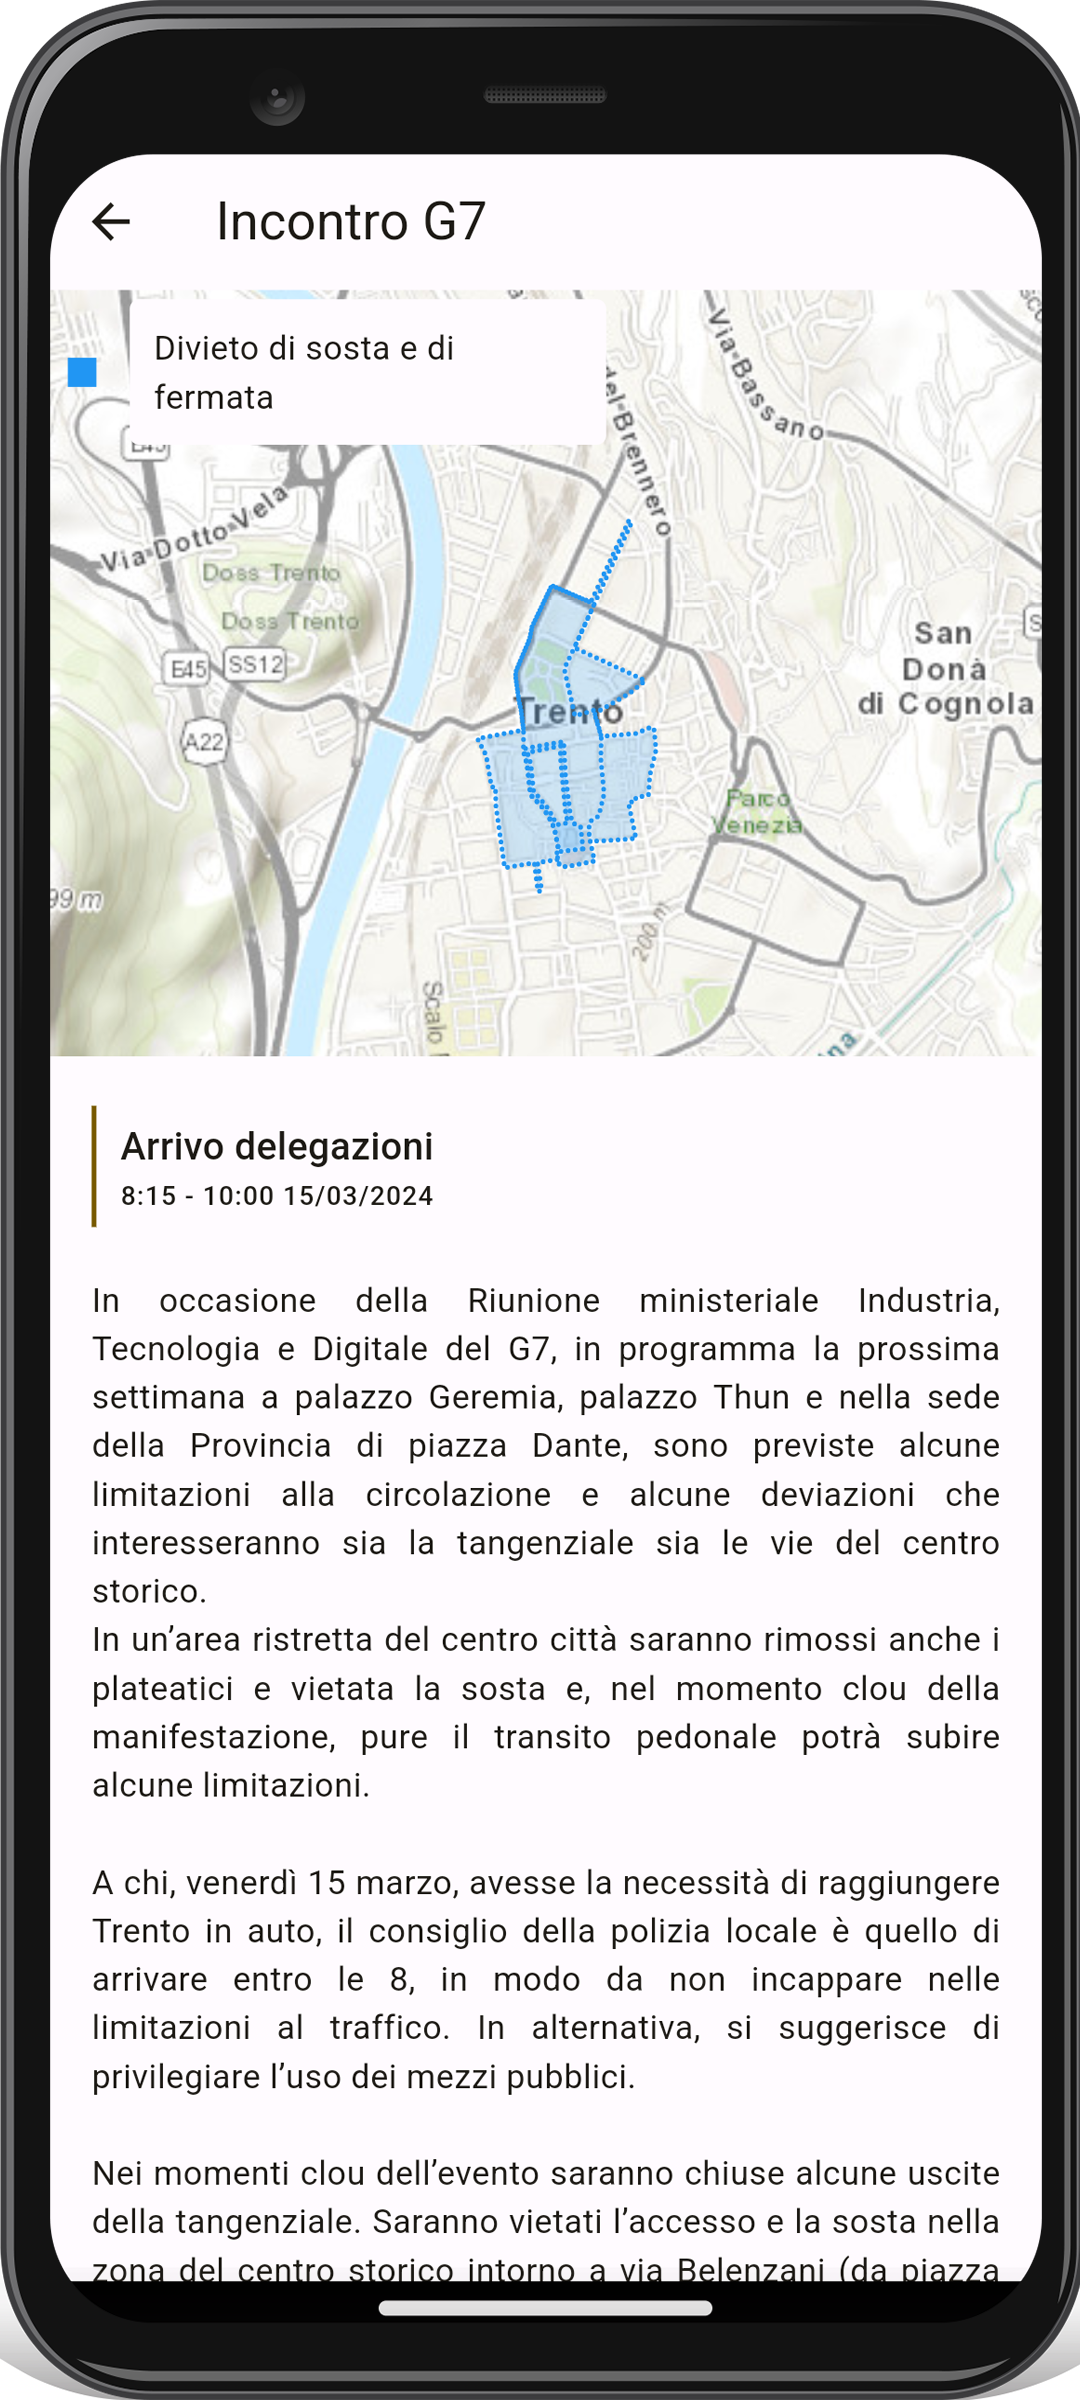
\includegraphics[width=0.25\textwidth]{Images/Mockup2 - Mobile.png}
    \caption{Mockup schermata detagli di un evento dell'applicazione mobile}
\end{figure}

In questo caso invece è riportata la schermata di visualizzazione dei dettagli di una variazione della viabilità.\\
È stato selezionato il precedente evento "Incontro G7", quindi sono visualizzati tutti i dettagli relativi a tale evento.\\
Nella fattispecie sono presenti la descrizione dell'evento, la data di inizio e fine, la zona interessata e la mappa con la visualizzazione della zona interessata.\\
Inoltre è presente un pulsante per tornare alla schermata principale dell'applicazione.\\
\clearpage

\subsubsection{Mockup notifiche degli eventi}
\index{Mockup notifiche degli eventi} % Aggiunge una voce all'indice

\begin{figure}[htbp]
    \label{fig:Notifica_evento}
    \centering
    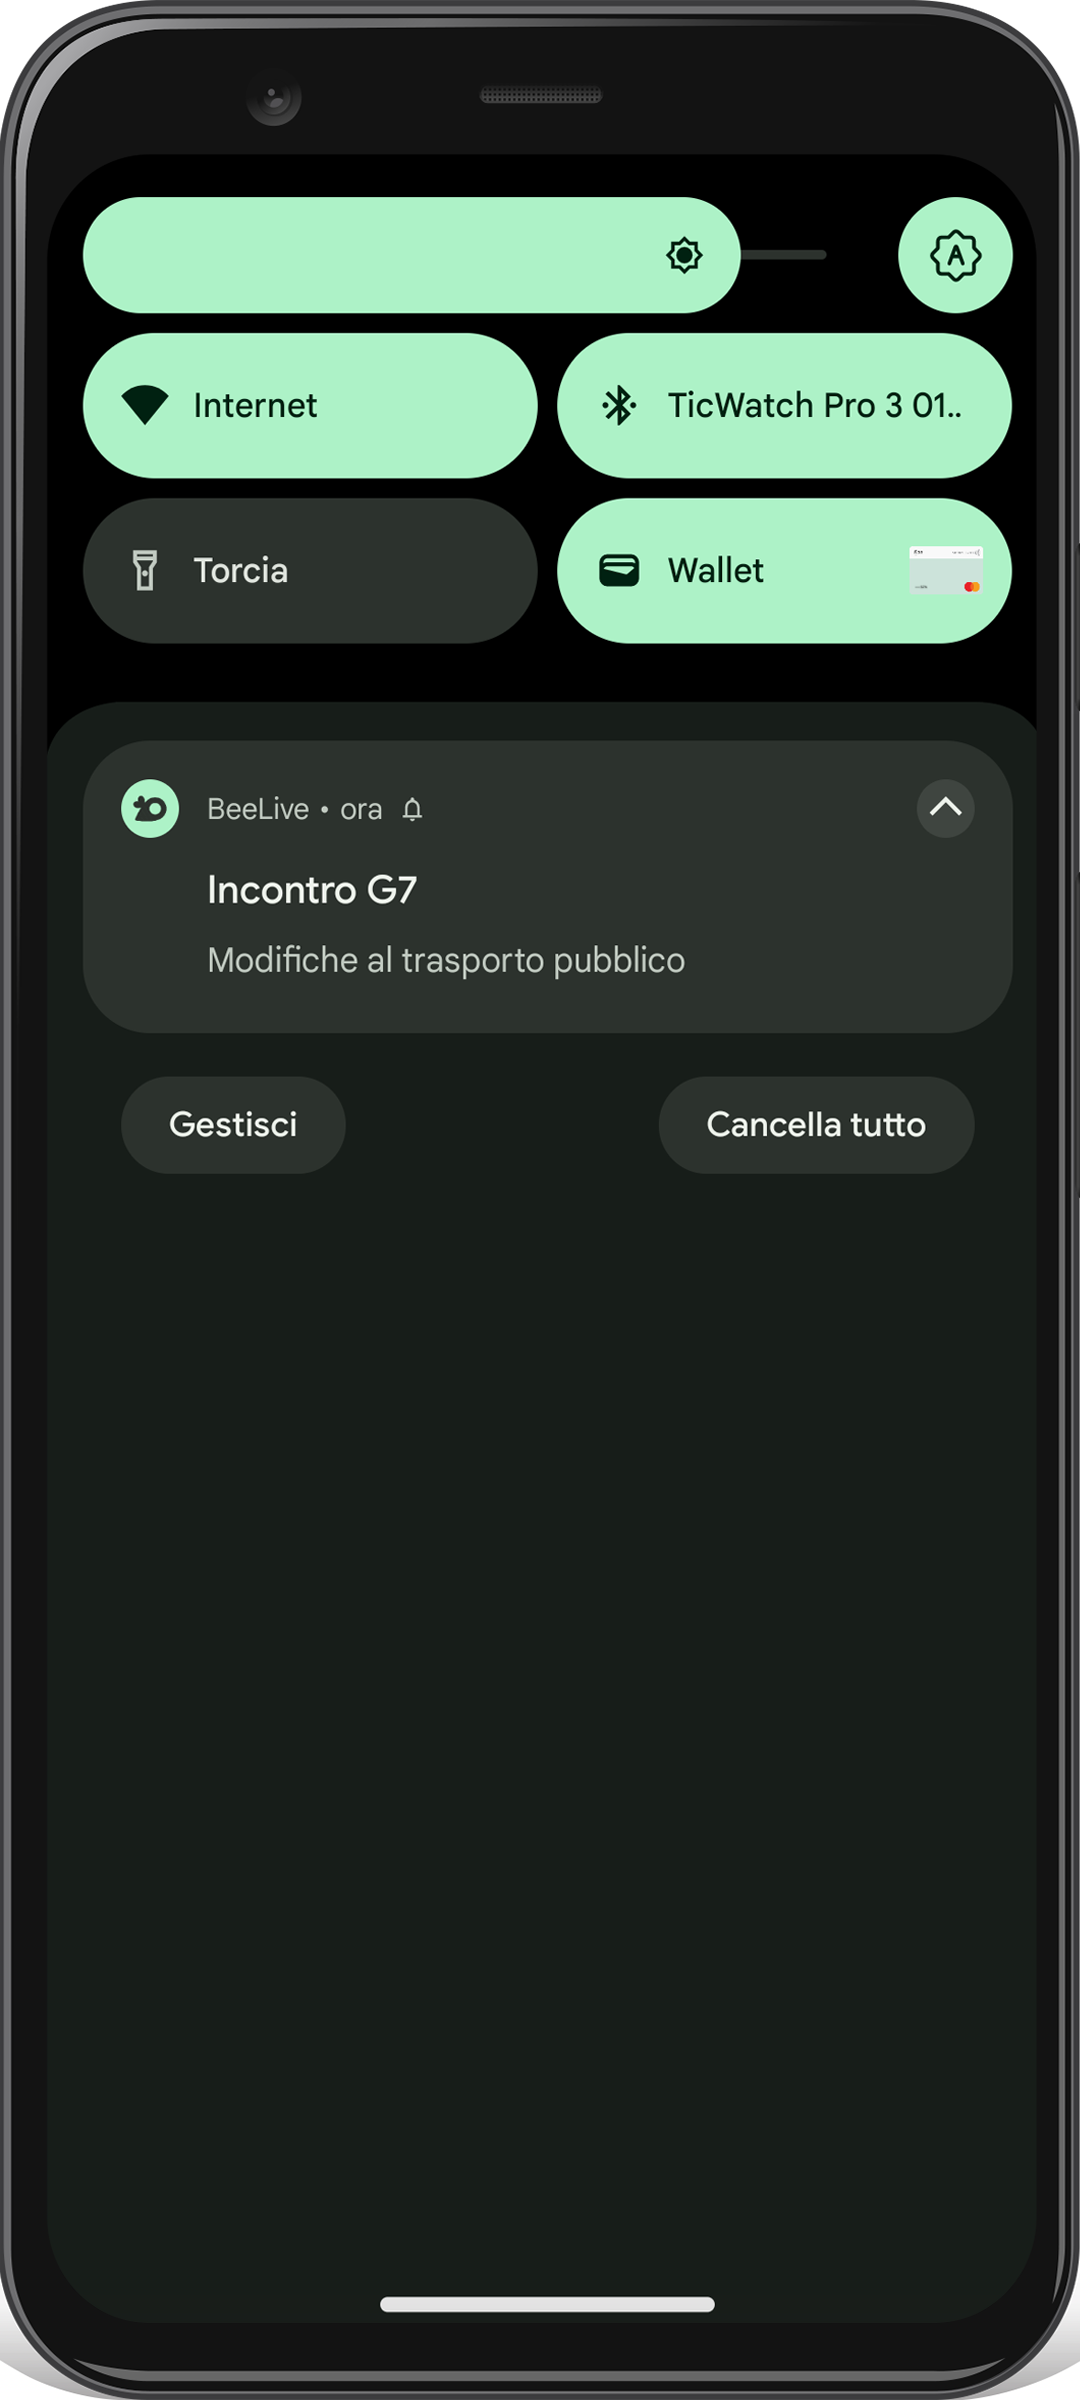
\includegraphics[width=0.25\textwidth]{Images/Mockup3 - Mobile.png}
    \caption{Mockup notifiche generate da un'evento dall'applicazione mobile}
\end{figure}

L'evento preso nell'esempio precedente era impostato per generare delle notifiche push.\\
Quella riportata nell'esempio soprastante rappresenta la notifica di inizio dell'evento "Incontro G7".\\
Interagendo con essa sarà quindi aperta l'applicazione mobile sulla schermata riportata in \hyperref[fig:Dettaglio_evento]{figura 2}, permettendo quindi la consultazione delle modifiche per intero.\\

\clearpage

\subsection{Mockup interfaccia desktop}
\index{Mockup interfaccia desktop} % Aggiunge una voce all'indice
%Immagine singola
\begin{figure}[htbp]
    \label{fig:Schermata_principale_desktop}
    \centering
    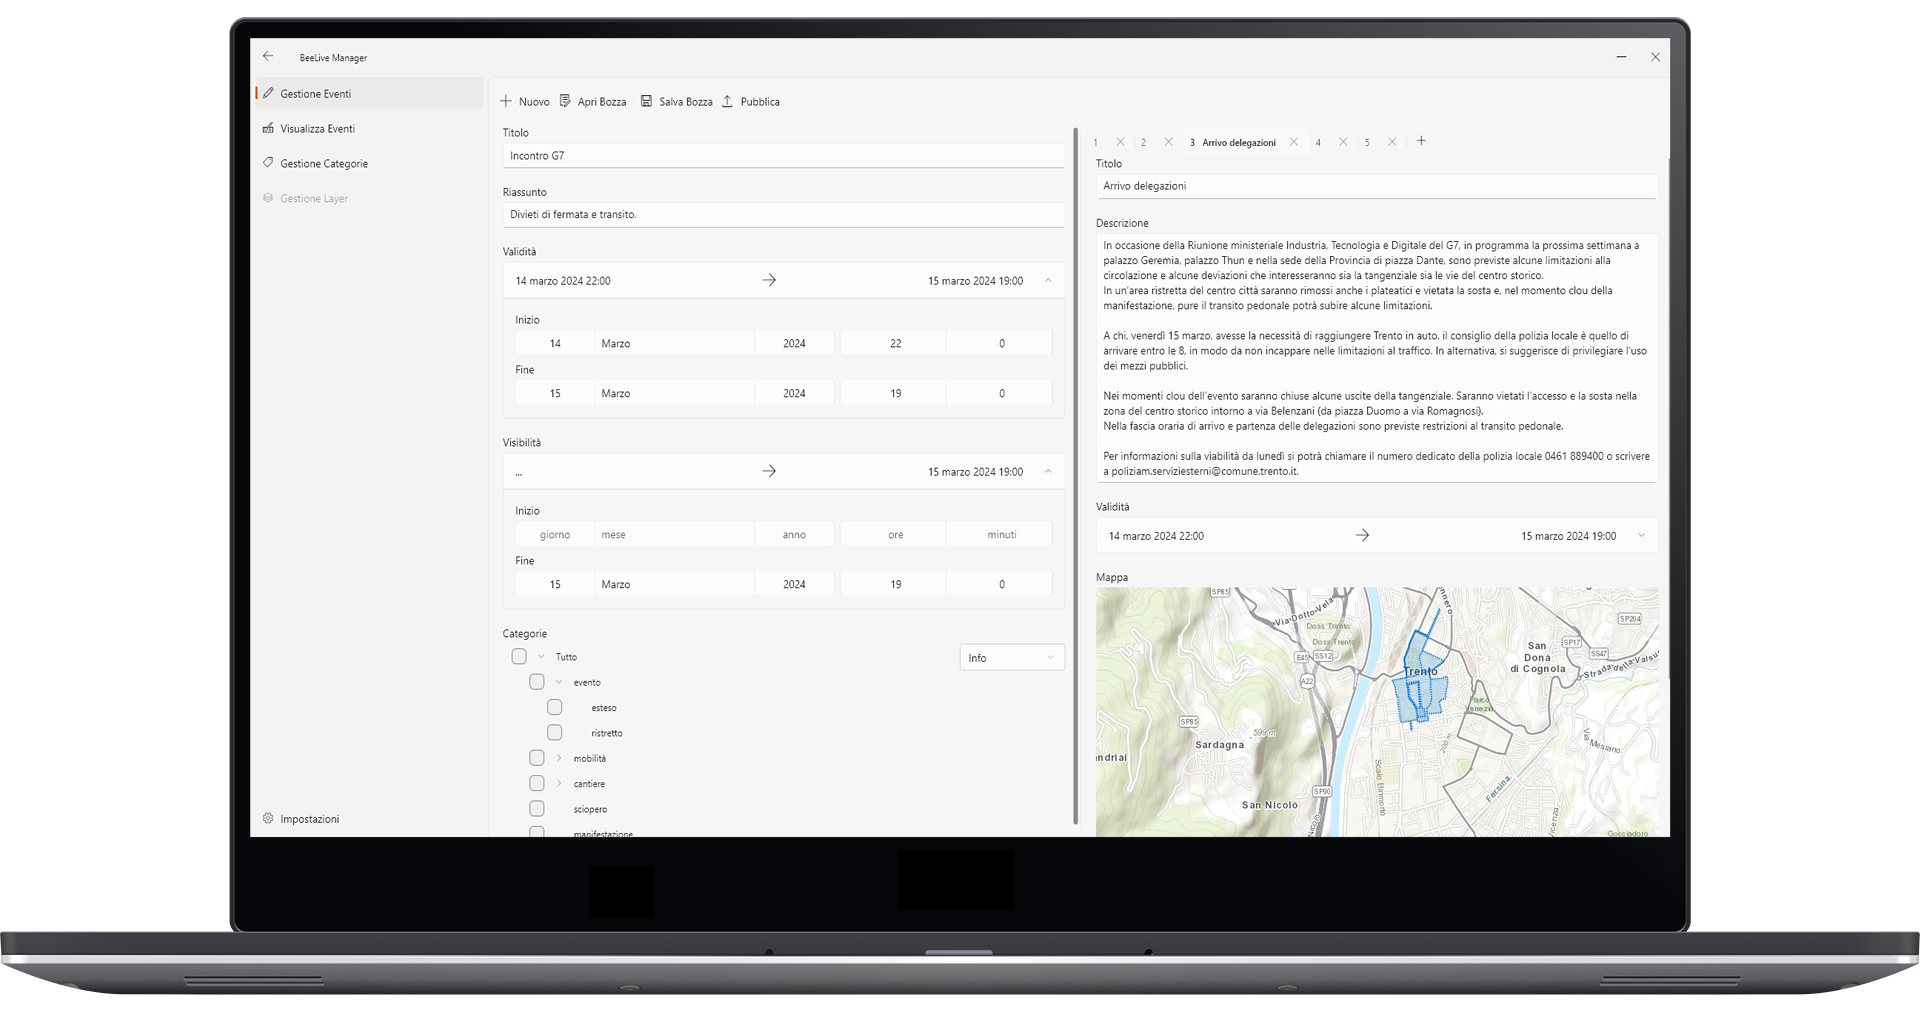
\includegraphics[width=0.75\textwidth]{Images/Mockup1 - Desktop.png}
    \caption{Mockup dell'interfaccia amministrativa}
\end{figure}

L'immagine rappresenta come dovrebbe essere strutturata l'interfaccia dell'applicativo desktop, utilizzato dagli enti pubblici con potere di amministrazione per la pobblicazione degli eventi in città che ne influenzano la viabilità.\\
L'interfaccia comprende un menu laterale per la navigazione tra le varie sezioni dell'applicativo e la schermata dove il sottomen selezionato presenta tutte le sue specifiche funzionalità disponibili.

Il sottomenù selezionato in questo caso è "Gestione Eventi", la sezione in cui è possibile inserire un nuovo evento che modifica la viabilità cittadina. Infatti sono riportati tutti i campi necessari per la creazione di un evento, come il titolo, il riassunto, la data di inizio e fine di validità dell'evento e di visibilità sull'applicativo mobile, e le categorie che caratterizzano l'evento.

L'interfaccia è strutturata in modo che ogni evento abbia la possibilità di essere composto da più sottoeventi. Nella sezione di destra è possibile visualizzare l'inderimento del sottoevento "Arrivo delle delegazioni", dove è possibile inserire il titolo, la descrizione, la data di validità e la zona interessata direttamente su mappa.\\

\clearpage

\section{Requisiti Funzionali}
\index{Requisiti funzionali}

\subsection{Utente anonimo tramite applicativo mobile}
\index{Utente anonimo tramite applicativo mobile} % Aggiunge una voce all'indice

\subsubsection{Deve poter visualizzare la lista degli eventi}\label{Requirements:Lista}
\index{Deve poter visualizzare la lista degli eventi} % Aggiunge una voce all'indice
L'utente anche se non autenticato a sistema deve avere la possibilità di visualizzare la lista intera di tutti gli eventi pubblicati.

\subsubsection{Deve poter filtrare gli eventi per categoria}
\index{Deve poter filtrare gli eventi per categoria} % Aggiunge una voce all'indice
Gli eventi sono divisi in categorie, l'utente deve avere la possibilità di esprimere le proprie preferenze sugli eventi da visualizzare in lista definita in \ref{Requirements:Lista}.

\subsubsection{Deve poter nascondere eventi specifici che non gli interessano}
\index{Deve poter nascondere eventi specifici che non gli interessano} % Aggiunge una voce all'indice
In caso l'utente non dimostri interesse per un evento specifico, deve avere la possibilità di nasconderlo dalla lista degli eventi.

\subsubsection{Deve poter visualizzare gli eventi su mappa}
\index{Deve poter visualizzare gli eventi su mappa} % Aggiunge una voce all'indice
L'utente deve essere in grado di visualizzare in modo intuitivo l'area fisica interessata dagli eventi di suo interesse. 

\subsubsection{Deve potersi registrare senza perdita di impostazioni}
\index{Deve potersi registrare senza perdita di impostazioni} % Aggiunge una voce all'indice
Le impostazioni selezionate da un utente anonimo non devono essere perse nel caso in cui questo si registri a sistema.

\subsubsection{Deve potersi autenticare}
\index{Deve potersi autenticare} % Aggiunge una voce all'indice
Gli utenti devono avere la possibilità di autenticarsi a sistema per usufruire della sincronizzazione tra dispositivi.

\subsubsection{Deve poter indicare categorie di interesse}
\index{Deve poter indicare categorie di interesse} % Aggiunge una voce all'indice
Deve poter indicare categorie di interesse in maniera indipendente per eventi in \textit{zone di interesse} (Aree e percorsi) e non.
\begin{itemize}
    \item Granularità maggiori (ad esempio: per zona di interesse e per label di rischio) non sono previste, in quanto \textbf{rischiano} di compromettere l'user experience
\end{itemize}

\subsubsection{Deve poter indicare aree di interesse}
\index{Deve poter indicare aree di interesse} % Aggiunge una voce all'indice
L'utente deve poter indicare delle zone su mappa per cui dimostra più interesse.

\subsubsection{Deve poter indicare percorsi di interesse}
\index{Deve poter indicare percorsi di interesse} % Aggiunge una voce all'indice
L'utente deve poter indicare dei percorsi su mappa per cui dimostra più interesse.

\subsubsection{Deve poter ricevere notifiche riguardo agli eventi}
\index{Deve poter ricevere notifiche riguardo agli eventi} % Aggiunge una voce all'indice
L'utente deve poter essere notificato all'insorgere determinati eventi.

\subsection{Utente autenticato tramite applicativo mobile}
\index{Utente autenticato tramite applicativo mobile} % Aggiunge una voce all'indice

\subsubsection{Deve avere le impostazioni sincronizzate tra i vari dispositivi}
\index{Deve avere le impostazioni sincronizzate tra i vari dispositivi} % Aggiunge una voce all'indice
Siccome l'utente autenticato tramite applicativo mobile eredita le caratteristiche dell'utente anonimo, valgono tutti i suoi requisiti, con l'aggiunta che in questo caso l'utente ha tutte le impostazioni sincronizzate su tutti i dispositivi in cui è autenticato.

\subsubsection{Non deve avere altri vantaggi rispetto l'utente non autenticato}
\index{Non deve avere altri vantaggi rispetto l'utente non autenticato} % Aggiunge una voce all'indice
L'applicativo deve poter essere utilizzato in maniera completa senza forzare l'autenticazione dell'utente, che ne comporta una barriera d'utilizzo, salvo evetuali problematiche implementative.

\subsection{Dipendente autorizzato del Comune di Trento tramite applicativo desktop}
\index{Dipendente autorizzato del Comune di Trento tramite applicativo desktop} % Aggiunge una voce all'indice

\subsubsection{Deve poter definire sottocategorie}
\index{Deve poter definire sottocategorie}
Le categorie sono organizzate in modo gerarchico per migliorare la granularità di filtraggio.

\subsubsection{Deve poter gestire gli eventi di sua competenza}
\index{Deve poter gestire gli eventi di sua competenza}
La gestione degli eventi di un dipendente include la creazione, la modifica, l'eliminazione e la pubblicazione (Solo se \textit{trusted}) degli eventi di sua competenza.

\subsubsection{Non deve poter gestire gli eventi che non sono di sua competenza}
\index{Non deve poter gestire gli eventi che non sono di sua competenza}
Il dipendente ha accesso solamente alle operazioni riguardanti gli eventi di sua competenza e non può gestire tutti gli altri.

\subsubsection{Deve poter risalire al dipendente autorizzato che ha gestito un evento specifico}
\index{Deve poter risalire al dipendente autorizzato che ha gestito un evento specifico}
Deve sempre essere possibile inividuare gli utenti autorizzati dal comune che hanno eseguito azioni sugli eventi pubblicati a sistema.

\subsubsection{Deve poter visionare lo storico della gestione degli eventi}
\index{Deve poter visionare lo storico della gestione degli eventi}
L'utente autorizzato deve poter visionare lo storico delle interazioni sugli eventi, con la possibilità di visionare chi ha effettuato l'attività e quando.

\subsubsection{Deve poter definire elementi geografici di interesse per facilitare la selezione delle aree interessate all'evento}
\index{Deve poter definire elementi geografici di interesse per facilitare la selezione delle aree interessate all'evento}
Per facilitare la selezione delle aree interessate all'evento, l'utente autorizzato deve poter definire elementi geografici notevoli.

\subsubsection{Deve poter sospendere la gestione di un evento e riprenderla successivamente}
\index{Deve poter sospendere la gestione di un evento e riprenderla successivamente}
Si deve avere la possibilità di sospendere la gestione di un evento, potendola riprendere successivamente senza alcuna perdita di dati.

\subsubsection{Deve poter caricare elementi geografici provenienti da file esterni}
\index{Deve poter caricare elementi geografici provenienti da file esterni}
L'utente, in fase di pubblicazione di un nuovo evento, deve avere la possibilità di indicare la zona d'interesse tramite il caricamento di un file contenente tutte le sue informazioni geografiche.

\subsubsection{Deve poter creare un evento a partire da file di strutture specifiche}
\index{Deve poter creare un evento a partire da file con strutture specifiche}
I dipartimenti devono poter continuare ad utilizzare i loro file attuali che determinano e caratterizzano gli eventi per la loro gestione sul sistema.

\subsubsection{Deve avere esclusività di gestione durante il corso dell'operazione}
\index{Deve avere esclusività di gestione durante il corso dell'operazione}
Durante l'operazione di gestione di un evento, l'utente deve avere l'esclusività di gestione, impedendo ad altri utenti di effettuare modifiche.

\subsection{Enti delegati tramite API gestionali del Web Server}
\index{Enti delegati tramite API gestionali del Web Server}
Questo attore eredita le capacità di "Dipendente autorizzato del Comune di Trento", integrandone le caratteristiche.

\subsection{Amministratore di sistema}
\index{Amministrazione di sistema}

\subsubsection{Deve poter gestire le policies di access control}
\index{Deve poter gestire le policies di access control}
Essendo l'amministratore di sistema, ha il compito di gestire tutte le policies di access control del sistema.

\subsubsection{Deve poter definire le aree di competenza delle entità di gestione}
\index{Deve poter definire le aree di competenza delle entità di gestione}
È compito suo definire tutte le aree di competenza di Dipendenti autorizzati del comune e Enti delegati.

\subsubsection{Deve avere accesso privilegiato al sistema}
\index{Deve avere accesso privilegiato al sistema}
Deve avere libertà nell'apportare modifiche specifiche alle componenti (Come il salvataggio dei dati)

\subsubsection{Deve poter definire le entità di gestione come \textit{trusted} o \textit{un-trusted}}
\index{Deve poter definire le entità di gestione come \textit{trusted} o \textit{un-trusted}}
È necessaria questa distinzione, solamente gli utenti \textit{trusted} possono accedere ai servizi offerti dal sistema.

\subsection{WebServer}
\index{WebServer}

\subsubsection{Deve garantire l'accesso al servizio ai soli utenti autorizzati}
\index{Deve garantire l'accesso al servizio ai soli utenti autorizzati}
Solamente gli utenti autorizzati (Anche i non autenticati, solo per alcuni servizi) possono accedere al servizio.

\subsection{DataBase}
\index{DataBase}

\subsubsection{Deve poter eseguire query spaziali}
\index{Deve poter eseguire query spaziali}
Sul DataBase sono salvati anche dati caratterizzati da coordinate. Deve essere possibile eseguire operazioni di ricerca su di esse.

\clearpage

\section{Requisiti non funzionali}
\index{Requisiti non funzionali} % Aggiunge una voce all'indice

\subsubsection{Affidabilità dei dati forniti}
\index{Affidabilità dei dati forniti}
Tutti i dati che provengono dagli enti delegati devono essere considerati affidabili dal resto del sistema.

\subsubsection{Usabilità}
\index{Usabilità} % Aggiunge una voce all'indice
Per quanto riguarda l'applicazione mobile, i cittadini devono essere in grado di utilizzarla dal primo momento in cui è intallata sul dispositivo.\\
Per invece l'applicativo desktop, precedentemente al primo utilizzo è necessaria al più una specificazione delle funzionalità per il loro completo utilizzo.

\subsubsection{Scalabilità}
\index{Scalabilità} % Aggiunge una voce all'indice
Il requirement di scalabilità riguarda solamente l'applicazione mobile, perchè deve essere in grado di gestire un elevato numero di utenti, che rispecchi il numero dgli abitanti di Trento.\\
L'applicativo desktop invece non ha bisogno di scalabilità, in quanto è utilizzato solo da un numero limitato di utenti.

\subsubsection{Robustness}
\index{Robustness} % Aggiunge una voce all'indice
Un guasto al webserver di visualizzazione non deve compromettere il funzionamento del webserver di gestione, e viceversa.

\subsubsection{Prestazioni di notifica}
\index{Prestazioni di notifica} % Aggiunge una voce all'indice
La notifica di un nuovo evento deve raggiungere tutti i dispositivi mobili, connessi ad internet e con l'applicazione installata, entro un tempo di 10 minuti

\subsubsection{Reliability}
\index{Reliability} % Aggiunge una voce all'indice
Il sistema non deve essere soggetto a errori imprevisti di alcun tipo, ed eventuali bug non devono compromettere eventuali dati sensibili presenti sul server.\\
Il sistema gestionale usato dagli utenti autorizzati non deve essere soggetto a vulnerabilità che ne compromettano la sicurezza. 

\subsubsection{WebServer diviso}
\index{WebServer diviso}
Ci sono due webserver, uno inerente il gestionale desktop e uno per gestire l'aplicazione mobile.

\subsubsection{Tipologia di DataBase}
\index{Tipologia di DataBase}
Deve essere utilizzato il DataBase non relazionale MongoDB.

\clearpage

\section{Grafo BPMN}
\index{Grafo BPMN} % Aggiunge una voce all'indice
\clearpage

\section{Casi d'uso}
\index{Casi d'uso} % Aggiunge una voce all'indice

\subsection{Utente anonimo}
\index{Utente anonimo}

\subsubsection{Registrazione ed autenticazione dell' utente anonimo}
\index{Registrazione ed autenticazione dell' utente anonimo}

\begin{table}[htbp]
    \centering
    \begin{tabularx}{\textwidth}{| l | p{0.795\textwidth} |}
        \Xhline{2pt} % Linea spessa
        Nome caso d'uso & Registrazione ed autenticazione dell' utente anonimo \\
        \Xhline{2pt} % Linea spessa
        ID & 001 \\
        \hline
        Descrizione & L'utente decide di creare un nuovo account all'interno del sistema oppure di accedere all'account precedentemente creato\\
        \hline
        Attori primari & Utente anonimo \\
        \hline
        Attori secondari & Server di autenticazione \\
        \hline
        Precondizioni & Nessuna \\
        \hline
        Flusso principale & 
            \begin{enumerate}
                \item Va aperto l'applicativo mobile
                \item Va selezionata l'opzione di accesso
                \item Il sistema reindirizza l'utente al form di registrazione dell'autenticatore esterno
                \item Se la registrazione va a buon fine:
                \begin{enumerate}
                    \item Se l'utente si è registrato:
                    \begin{enumerate}
                        \item Viene creato il profilo
                        \item Vengono sincronizzate tutte le preferenze utente
                    \end{enumerate}
                    \item L'utente diventa un utente autenticato
                \end{enumerate}
                \item Altrimenti:
                \begin{enumerate}
                    \item L'utente rimane anonimo.
                \end{enumerate}
            \end{enumerate}
        \\
        \hline
    \end{tabularx}
    \caption{Registrazione ed autenticazione dell' utente anonimo}
    \label{tab:tabella_use_case001}
\end{table}

\clearpage

\subsection{Utente anonimo o autenticato}
\index{Utente anonimo o autenticato}

\subsubsection{Visualizzazione degli eventi}
\index{Visualizzazione degli eventi}

\begin{table}[htbp]
    \centering
    \begin{tabularx}{\textwidth}{| l | p{0.795\textwidth} |}
        \Xhline{2pt} % Linea spessa
        Nome caso d'uso & Visualizzazione degli eventi \\
        \Xhline{2pt} % Linea spessa
        ID & 002 \\
        \hline
        Descrizione & L'utente intende visualizzare gli eventi disponibili\\
        \hline
        Attori primari & Utente anonimo o autenticato\\
        \hline
        Attori secondari & Nessuno \\
        \hline
        Precondizioni & Nessuna \\
        \hline
        Flusso principale & 
            \begin{enumerate}
                \item Va aperto l'applicativo mobile
                \item Se non vi è connettività internet
                \begin{enumerate}
                    \item Viene mostrato un banner che indica la mancanza di connessione
                \end{enumerate}
            \end{enumerate}
        \\
        \hline
    \end{tabularx}
    \caption{Visualizzazione degli eventi}
    \label{tab:tabella_use_case002}
\end{table}

\subsubsection{Visualizzazione dei dettagli di un evento}
\index{Visualizzazione dei dettagli di un evento}

\begin{table}[htbp]
    \centering
    \begin{tabularx}{\textwidth}{| l | p{0.795\textwidth} |}
        \Xhline{2pt} % Linea spessa
        Nome caso d'uso & Visualizzazione dei dettagli \\
        \Xhline{2pt} % Linea spessa
        ID & 003 \\
        \hline
        Descrizione & L'utente intende visualizzare i dettagli di un evento specifico\\
        \hline
        Attori primari & Utente anonimo o autenticato\\
        \hline
        Attori secondari & Nessuno \\
        \hline
        Precondizioni & Nessuna \\
        \hline
        Flusso principale & 
            \begin{enumerate}
                \item Se si riceve una notifica push
                \begin{enumerate}
                    \item L'utente interagisce con la notifica
                \end{enumerate}
                \item Altrimenti
                \begin{enumerate}
                    \item Va aperto l'applicativo mobile
                    \item Viene selezionato un evento dalla lista
                \end{enumerate}
                \item Viene visualizzata la schermata dei dettagli
            \end{enumerate}
        \\
        \hline
    \end{tabularx}
    \caption{Visualizzazione dei dettagli di un evento}
    \label{tab:tabella_use_case003}
\end{table}

\clearpage

\subsubsection{Filtraggio degli eventi}
\index{Filtraggio degli eventi}

\begin{table}[htbp]
    \centering
    \begin{tabularx}{\textwidth}{| l | p{0.795\textwidth} |}
        \Xhline{2pt} % Linea spessa
        Nome caso d'uso & Filtraggio degli eventi \\
        \Xhline{2pt} % Linea spessa
        ID & 004 \\
        \hline
        Descrizione & L'utente intende filtrare gli eventi disponibili\\
        \hline
        Attori primari & Utente anonimo o autenticato\\
        \hline
        Attori secondari & Nessuno \\
        \hline
        Precondizioni & Nessuna \\
        \hline
        Flusso principale & 
            \begin{enumerate}
                \item Viene aperto l'applicativo mobile
                \item Se l'utente desidera effettuare una selezione temporanea
                \begin{enumerate}
                    \item Interagisce con il filtraggio delle categorie su mappa
                \end{enumerate}
                \item Altrimenti
                \begin{enumerate}
                    \item Sono aperte le impostazioni
                    \item L'utente seleziona le categorie di suo interesse
                \end{enumerate}
            \end{enumerate}
        \\
        \hline
        Postcondizioni & Vengono visualizzati solamente gli eventi selezionati \\
        \hline
    \end{tabularx}
    \caption{Visualizzazione degli eventi}
    \label{tab:tabella_use_case004}
\end{table}

\subsubsection{Selezione dei percorsi di interesse}
\index{Selezione dei percorsi di interesse}

\begin{table}[htbp]
    \centering
    \begin{tabularx}{\textwidth}{| l | p{0.795\textwidth} |}
        \Xhline{2pt} % Linea spessa
        Nome caso d'uso & Selezione dei percorsi di interesse \\
        \Xhline{2pt} % Linea spessa
        ID & 005 \\
        \hline
        Descrizione & L'utente va a selezionare i percorsi di suo interesse\\
        \hline
        Attori primari & Utente anonimo o autenticato\\
        \hline
        Attori secondari & Nessuno \\
        \hline
        Precondizioni & Nessuna \\
        \hline
        Flusso principale & 
            \begin{enumerate}
                \item Va aperta l'applicazione mobile
                \item Viene aperta la sezione di impostazioni
                \item L'utente va a selezionare in modalità interattiva il percorso d'interesse
            \end{enumerate}
        \\
        \hline
        Postcondizioni & Il percorso selezionato viene salvato su database \\
        \hline
    \end{tabularx}
    \caption{Selezione dei percorsi di interesse}
    \label{tab:tabella_use_case004}
\end{table}

\clearpage

\subsubsection{Selezione delle aree di interesse}
\index{Selezione delle aree di interesse}

\begin{table}[htbp]
    \centering
    \begin{tabularx}{\textwidth}{| l | p{0.795\textwidth} |}
        \Xhline{2pt} % Linea spessa
        Nome caso d'uso & Selezione delle aree di interesse \\
        \Xhline{2pt} % Linea spessa
        ID & 005 \\
        \hline
        Descrizione & L'utente va a selezionare le aree di suo interesse\\
        \hline
        Attori primari & Utente anonimo o autenticato\\
        \hline
        Attori secondari & Nessuno \\
        \hline
        Precondizioni & Nessuna \\
        \hline
        Flusso principale & 
            \begin{enumerate}
                \item Va aperta l'applicazione mobile
                \item Viene aperta la sezione di impostazioni
                \item L'utente va a selezionare in modalità interattiva le aree di suo interesse
            \end{enumerate}
        \\
        \hline
        Postcondizioni & L'area selezionata viene salvata su database \\
        \hline
    \end{tabularx}
    \caption{Selezione dei percorsi di interesse}
    \label{tab:tabella_use_case004}
\end{table}



\subsection{Dipendente autorizzato del Comune di Trento}
\index{Dipendente autorizzato del Comune di Trento}

\subsubsection{Definizione delle sottocategorie}
\index{Definizione delle sottocategorie}

\begin{table}[htbp]
    \centering
    \begin{tabularx}{\textwidth}{| l | p{0.795\textwidth} |}
        \Xhline{2pt} % Linea spessa
        Nome caso d'uso & Definizione delle sottocategorie \\
        \Xhline{2pt} % Linea spessa
        ID & 005 \\
        \hline
        Descrizione & Il dipendente autorizzato del Comune di Trento vuole creare una nuova sottoategoria per eventi di sua competenza\\
        \hline
        Attori primari & Dipendente autorizzato del Comune di trento\\
        \hline
        Attori secondari & Nessuno \\
        \hline
        Precondizioni & Nessuna \\
        \hline
        Flusso principale & 
            \begin{enumerate}
                \item Va aperto l'applicativo desktop
                \item L'utente va a selezionare l'opzione \textit{Gestione Eventi}
                \item Procede con la compilazione di tutti i campi necessari alla creazione della sottocategoria
                \item Se la creazione va a buon fine:
                \begin{enumerate}
                    \item La nuova sottocategoria ssarà visibile a sistema
                \end{enumerate}
                \item Altrimenti:
                \begin{enumerate}
                    \item Sarà visualizzato un alert che avvisa dell'errore
                \end{enumerate}
            \end{enumerate}
        \\
        \hline
    \end{tabularx}
    \caption{Definizione delle sottocategorie}
    \label{tab:tabella_use_case006}
\end{table}

\clearpage

\subsubsection{Creazione degli eventi}
\index{Creazione degli eventi}

\begin{table}[htbp]
    \centering
    \begin{tabularx}{\textwidth}{| l | p{0.795\textwidth} |}
        \Xhline{2pt} % Linea spessa
        Nome caso d'uso & Creazione degli eventi \\
        \Xhline{2pt} % Linea spessa
        ID & 006 \\
        \hline
        Descrizione & Il dipendente autorizzato del Comune di Trento crea gli eventi di sua competenza\\
        \hline
        Attori primari & Dipendente autorizzato del Comune di trento\\
        \hline
        Attori secondari & Nessuno \\
        \hline
        Precondizioni & Nessuna \\
        \hline
        Flusso principale & 
            \begin{enumerate}
                \item Va aperto l'applicativo desktop
                \item È selezionata la sezione \textit{Gestione Eventi}
                \item Viene scelta la voce \textit{Nuovo Evento}
                \item Sono compilati tutti i campi che caratterizzano il nuovo evento
                \item L'evento viene salvato e/o pubblicato a sistema
                \item Se la creazione va a buon fine:
                \begin{enumerate}
                    \item L'evento verrà memorizzato (e comunicato tempestivamente)
                \end{enumerate}
                \item Altrimenti:
                \begin{enumerate}
                    \item Sarà visualizzato un alert che avvisa dell'errore
                \end{enumerate}
            \end{enumerate}
        \\
        \hline
    \end{tabularx}
    \caption{Creazione nuovi eventi}
    \label{tab:tabella_use_case006}
\end{table}

\clearpage

\subsubsection{Modifica di un evento}
\index{Modifica di un evento}

\begin{table}[htbp]
    \centering
    \begin{tabularx}{\textwidth}{| l | p{0.795\textwidth} |}
        \Xhline{2pt} % Linea spessa
        Nome caso d'uso & Modifica di un evento \\
        \Xhline{2pt} % Linea spessa
        ID & 007 \\
        \hline
        Descrizione & Il dipendente autorizzato del Comune di Trento intende modificare un evento di sua competenza\\
        \hline
        Attori primari & Dipendente autorizzato del Comune di trento\\
        \hline
        Attori secondari & Nessuno \\
        \hline
        Precondizioni & Nessuna \\
        \hline
        Flusso principale & 
            \begin{enumerate}
                \item Va aperto l'applicativo desktop
                \item È selezionata la sezione \textit{Visualizza Eventi} per visualizzare quelli disponibili a sistema
                \item Viene scelta l'icona di modifica
                \item Sono modificati i campi che il dipendente del Comune intende aggiornare
                \item L'evento viene salvato e/o pubblicato a sistema
                \item Se la modifica va a buon fine:
                \begin{enumerate}
                    \item L'evento verrà memorizzato (e comunicato tempestivamente)
                \end{enumerate}
                \item Altrimenti:
                \begin{enumerate}
                    \item Sarà visualizzato un alert che avvisa dell'errore
                \end{enumerate}
            \end{enumerate}
        \\
        \hline
    \end{tabularx}
    \caption{Modifica di un evento}
    \label{tab:tabella_use_case007}
\end{table}

\clearpage

\subsubsection{Modifica di un evento}
\index{Modifica di un evento}

\begin{table}[htbp]
    \centering
    \begin{tabularx}{\textwidth}{| l | p{0.795\textwidth} |}
        \Xhline{2pt} % Linea spessa
        Nome caso d'uso & Modifica di un evento \\
        \Xhline{2pt} % Linea spessa
        ID & 008 \\
        \hline
        Descrizione & Il dipendente autorizzato del Comune di Trento intende eliminare un evento di sua competenza\\
        \hline
        Attori primari & Dipendente autorizzato del Comune di trento\\
        \hline
        Attori secondari & Nessuno \\
        \hline
        Precondizioni & Nessuna \\
        \hline
        Flusso principale & 
            \begin{enumerate}
                \item Va aperto l'applicativo desktop
                \item È selezionata la sezione \textit{Visualizza Eventi} per visualizzare quelli disponibili a sistema
                \item Viene scelta l'icona di eliminazione dell'evento che si intende modificare
                \item Se la cancellazione va a buon fine:
                \begin{enumerate}
                    \item L'evento verrà eliminato dal sistema
                    \item Viene confermata l'eliminazione
                \end{enumerate}
                \item Altrimenti:
                \begin{enumerate}
                    \item Sarà visualizzato un alert che avvisa dell'errore
                \end{enumerate}
            \end{enumerate}
        \\
        \hline
    \end{tabularx}
    \caption{Eliminazione di un evento}
    \label{tab:tabella_use_case008}
\end{table}

\clearpage

\section{Diagramma dei casi d'uso}
\index{Diagramma dei casi d'uso} % Aggiunge una voce all'indice

\clearpage

\section{Resoconto}
\index{Resoconto} % Aggiunge una voce all'indice

Segue la tabella dei riferimenti, utile alla comprensione generale delle diverse sezioni riguardanti lo specifico obiettivo.\\

\begin{table}[htbp]
    \centering
    \begin{tabularx}{\textwidth}{|X|X|X|X|X|X|}
        \Xhline{2pt} % Linea spessa
        Obiettivo & Attore & User Story & Use Case\newline diagram & Requisiti\newline funzionali & Mockup \\
        \Xhline{2pt} % Linea spessa
        1 & 2 & 3 & 4 & 5 & 6 \\
        \hline
    \end{tabularx}
    \caption{Tabella riassuntiva}
    \label{tab:tabella_tutta_pagina}
\end{table}

\end{document}
